\clearpage
\VerdierPhysicalPageAnchor{0135}%
\begingroup
\normalsize
\setlength{\emergencystretch}{1.5em}%
\setlength{\abovedisplayskip}{2pt plus 1pt minus 1pt}%
\setlength{\belowdisplayskip}{2pt plus 1pt minus 1pt}%

\VerdierSemanticAnchor{ch2-2-2-1-x-backslash-s-diagram}
\noindent\hspace*{.3em}(それぞれ\quad
\begin{tikzpicture}[>=stealth,line width=.38pt,scale=.90,transform shape,
  baseline={(current bounding box.center)}]
  \node (X)  at (0,1.50) {$X$};
  \node (Y)  at (-1.30,-.55) {$Y$};
  \node (Yp) at (1.30,-.55) {$Y'$};
  \draw[->] (X) -- node[left=2pt] {$s$} (Y);
  \draw[->] (X) -- node[right=2pt] {$t$} (Yp);
  \draw[->] (Y) -- node[above=1pt] {$u$} (Yp);
  \node at (3.10,.45) {$s,t\in S$};
\end{tikzpicture}
\quad )\,.

\VerdierSemanticAnchor{ch2-2-2-1-localized-hom-definition}
\smallskip
\noindent $\mathcal C$ の対象の各対 $X,Y$ に対し、次のようにおく：

\VerdierSemanticAnchor{ch2-2-2-1-formula-2-2-1-1}
\par\smallskip
\noindent\makebox[0pt][l]{(2.2.1.1)}%
\begin{minipage}[t]{\linewidth}
  \centering
  $\displaystyle
    \operatorname{Hom}_{\mathcal C(S^{-1})}(X,Y)
    =\varinjlim_{(S/X)^{\circ}}
     \operatorname{Hom}_{\mathcal C}(\,\cdot\,,Y)\,.$
\end{minipage}
\par\smallskip

\VerdierSemanticAnchor{ch2-2-2-1-dot-explanation}
\noindent （式 (2.2.1.1) の「点」は $S/X$ の可変対象の始域を表す。）

\VerdierSemanticAnchor{ch2-2-2-1-filtered-category}
性質 SM1)、SM2)、SM3) から、圏 $(S/X)^{\circ}$ がフィルター圏 [6]
であることが直ちに従う。
\VerdierSemanticAnchor{ch2-2-2-1-roof-class}%
したがって $\operatorname{Hom}_{\mathcal C(S^{-1})}(X,Y)$ の元は、次の形の
図式の同値類である：

\VerdierSemanticAnchor{ch2-2-2-1-roof-formula}
\[
  D=X\xleftarrow{s}X'\xrightarrow{m}Y,\qquad s\in S,
\]

\VerdierSemanticAnchor{ch2-2-2-1-equivalence-setup}
\noindent 二つの図式
$D_1=X\xleftarrow{s_1}X_1\xrightarrow{m_1}Y$ と
$D_2=X\xleftarrow{s_2}X_2\xrightarrow{m_2}Y$ が同じ同値類に属するための
必要十分条件は、次の図式が存在することである：

\VerdierSemanticAnchor{ch2-2-2-1-common-refinement-roof}
\[
  D_3=X\xleftarrow{s_3}X_3\xrightarrow{m_3}Y,\qquad s_3\in S,
\]

\VerdierSemanticAnchor{ch2-2-2-1-common-refinement-diagram-introduction}
\noindent および次の可換図式：

\VerdierSemanticAnchor{ch2-2-2-1-common-refinement-diagram}
\begin{center}
  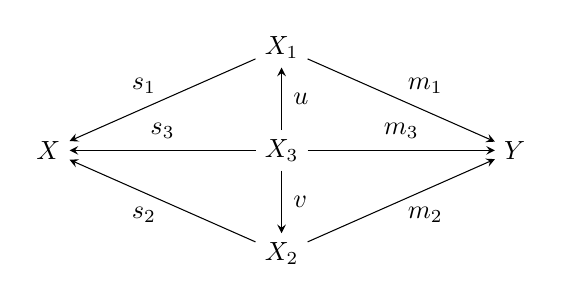
\begin{tikzpicture}[>=stealth,line width=.38pt,x=1.45cm,y=1.02cm,
    scale=.95,transform shape]
    \node (X1) at (0,1.35) {$X_1$};
    \node (X3) at (0,0) {$X_3$};
    \node (X2) at (0,-1.35) {$X_2$};
    \node (X)  at (-2.15,0) {$X$};
    \node (Y)  at (2.15,0) {$Y$};
    \draw[->] (X1) -- node[above left=-1pt] {$s_1$} (X);
    \draw[->] (X3) -- node[above=1pt] {$s_3$} (X);
    \draw[->] (X2) -- node[below left=-1pt] {$s_2$} (X);
    \draw[->] (X3) -- node[right=1pt] {$u$} (X1);
    \draw[->] (X3) -- node[right=1pt] {$v$} (X2);
    \draw[->] (X1) -- node[above right=-1pt] {$m_1$} (Y);
    \draw[->] (X3) -- node[above=1pt] {$m_3$} (Y);
    \draw[->] (X2) -- node[below right=-1pt] {$m_2$} (Y);
  \end{tikzpicture}
  \quad .
\end{center}

\VerdierSemanticAnchor{ch2-2-2-1-q-of-f}
\noindent 各元 $f\in\operatorname{Hom}_{\mathcal C}(X,Y)$ に対し、図式
$X\xleftarrow{\operatorname{id}_X}X\xrightarrow{f}Y$ の同値類を $Q(f)$
と書く。
\VerdierSemanticAnchor{ch2-2-2-1-q-of-s-inverse}%
各射 $s\colon Y\to X$、$s\in S$ に対し、図式
$X\xleftarrow{s}Y\xrightarrow{\operatorname{id}_Y}Y$ の同値類を
$Q(s)^{-1}$ と書く。

\VerdierSemanticAnchor{ch2-2-2-1-fl-morphism-set}
次に、$\operatorname{Fl}(\mathcal C(S^{-1}))$ により次の集合を表す：

\VerdierSemanticAnchor{ch2-2-2-1-fl-product-formula}
\[
  \prod_{(X,Y)\in\operatorname{Ob}(\mathcal C)\times\operatorname{Ob}(\mathcal C)}
  \operatorname{Hom}_{\mathcal C(S^{-1})}(X,Y),
\]

\VerdierSemanticAnchor{ch2-2-2-1-p136-boundary}
\endgroup
